\chapter{Results}
If we apply the finished algorithm to various test data sets, we can get an impression of what the program is capable of.
For each riddle beeing solved, the algorithms are executed a number of times to calculate an average runtime.\\
In both cases A$^\star$ was used as the search algorithm on the resulting graph. As a distance measurement the heuristic in form of the 2-norm of the vector between current position and target was added to the stepcount with each step weighting 0.1 units. The starting distance to beetween main object and target 10.1980 units.
\section{Measurements}
The algorithms are described as pList for the implementation with point lists and fList for the implementation with functions. The adaption of the algorithm to work with cells as node identification is called fCell.
\subsection{Rotation and Translation}
First the algorithm is tested against rotation and translation with one obstalce (blue). This object has a fixed position and only rotations are allowed.\\
The same riddle is then used and solved simply by translation with no rotation allowed for the obstacle. The main object (green) can rotate and move in both cases inside the border (black) to get to the target area (red).

\begin{figure}[H]
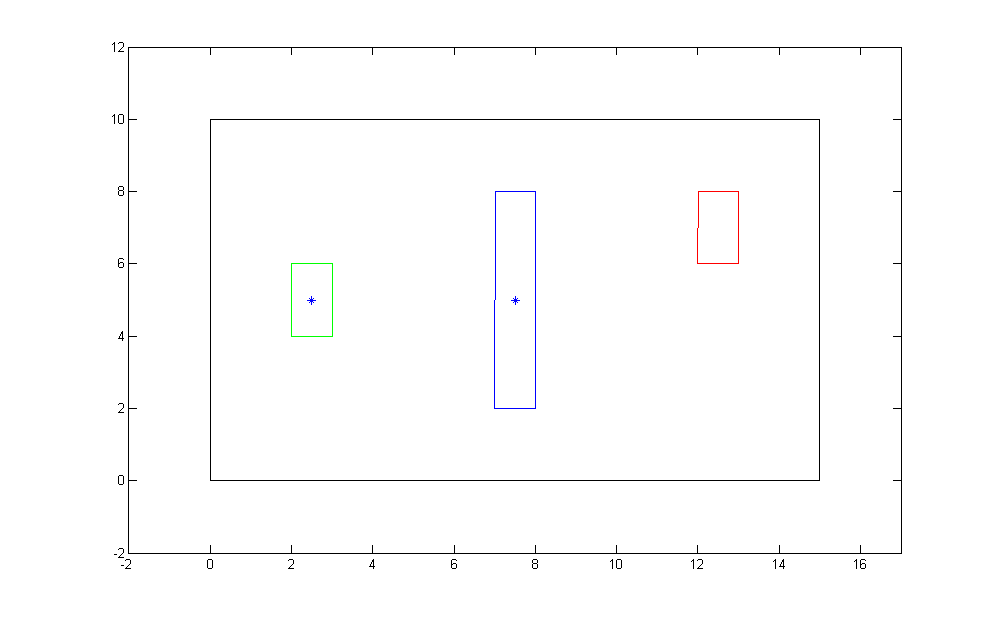
\includegraphics[scale = 0.5]{rotRiddle.png}
\centering
\caption{Riddle with main object, border, target and moveable obstacle.}
\end{figure}
\begin{table}[H]
\centering
\begin{tabular}{l||c|c|c||c|c|c}
& \multicolumn{3}{c||}{rotation} &\multicolumn{3}{c}{translation}\\\hline\hline
Algorithm& fastest & slowest & medium & fastest & slowest & medium\\\hline
pList &  18.8819 & 22.8457  & 21.0269 &  0.1211& 0.1272  & 0.1231\\
fList  & 0.1176&0.1635  &0.1296  & 0.0291 & 0.0504 & 0.0367 \\
fCell & 0.3404 & 0.4012 & 0.3698 & 0.2894 & 0.4112 & 0.3358 \\
\end{tabular}
\caption{Time in seconds for rotation riddle and translation riddle.}
\end{table}

\subsection{Small Riddles}
Two simple small riddles with 2 and 4 moveable obstacles.
\begin{figure}[H]
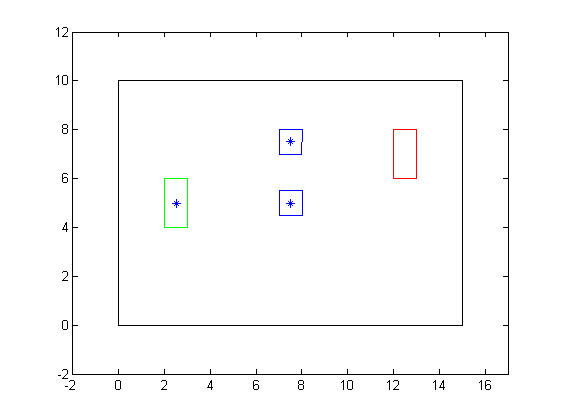
\includegraphics[scale = 0.5]{riddle2}
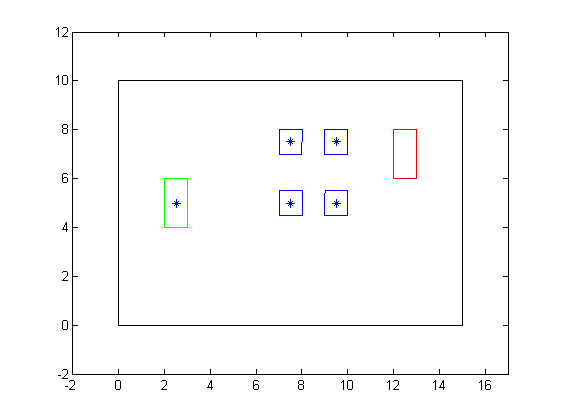
\includegraphics[scale = 0.5]{riddle4}
\caption{Riddle with two and four movable obstacles.}
\end{figure}
\begin{table}[H]
\centering
\begin{tabular}{l||c|c|c||c|c|c}
& \multicolumn{3}{c||}{2 objects} &\multicolumn{3}{c}{4 objects}\\\hline\hline
Algorithm& fastest & slowest & medium & fastest & slowest & medium\\\hline
pList & 4.7801& 5.1930&4.9305& 85.1726 & 90.9629 & 89.3621\\
fList  & 0.6242 & 0.8082& 0.6747  & 7.3608 & 8.1557 & 7.7242\\
fCell & 0.1362 & 0.1591 & 0.1472 & 13.2560 & 14.0114 & 13.5623\\
\end{tabular}
\caption{Time in seconds for small riddle with 2 and 4 obstacles.}
\end{table}
% cell times 2 | 4
% avg 0.1285| 6.2646
% min 0.1267| 6.1976
%max 0.1320| 6.3642

\subsection{Medium Riddles}
Bigger riddle with 6 and 8 moveable obstacles.\\
\begin{figure}[H]
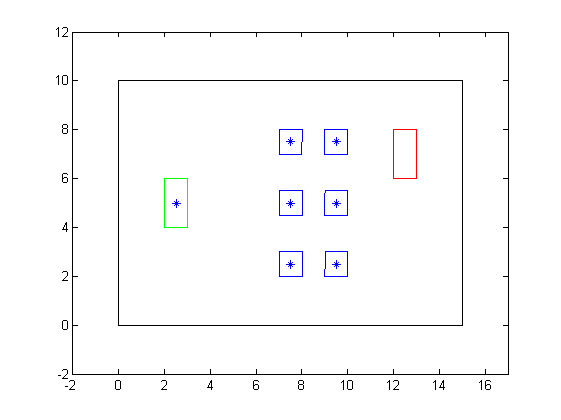
\includegraphics[scale = 0.5]{riddle6}
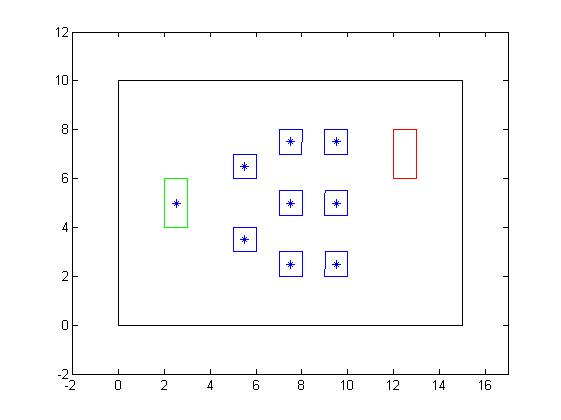
\includegraphics[scale = 0.5]{riddle8}
\caption{Riddle with six and eight moveable obstacles.}
\end{figure}
\begin{table}[H]
\centering
\begin{tabular}{l||c|c|c||c|c|c}
& \multicolumn{3}{c||}{6 objects} &\multicolumn{3}{c}{8 objects}\\\hline\hline
Algorithm& fastest & slowest & medium & fastest & slowest & medium\\\hline
pList &  395.0670 & 415.7986 & 403.9329  & 1790.5 &1972.5 &1855.4\\
fList  &  32.6039 &  34.4411 & 33.7001 & 30.4606 & 33.9077 & 32.1049\\
fCell & 49.1205 & 51.2846 & 50.3155 & 95.5828 & 106.6468 & 100.63497\\
\end{tabular}
\caption{Time in seconds for medium riddle with 6 and 8 obstacles.}
\end{table}

%\subsection{Large riddles}
%Large riddle with 12 and 16 moveable obstacles.\\
%\begin{figure}[H]
%%\includegraphics[scale = 0.5]{riddle12}
%%\includegraphics[scale = 0.5]{riddle16}
%\caption{Riddle with twelve and sixteen moveable obstacles.}
%\end{figure}
%\begin{table}[H]
%\centering
%\begin{tabular}{l||c|c|c||c|c|c}
%& \multicolumn{3}{c||}{12 objects} &\multicolumn{3}{c}{16 objects}\\\hline\hline
%Algorithm& fastest & slowest & medium & fastest & slowest & medium\\\hline
%pList &  - & - & -  & - &- &-\\
%fList  &  32.6039 &  34.4411 & 33.7001 & 30.4606 & 33.9077 & 32.1049\\
%fCell & 251.4319 & 395.3441 & 305.9431 & 79.4915 & 108.6652 & 102.6317\\
%\end{tabular}
%\caption{Time in seconds for medium riddle with 6 and 8 obstacles.}
%\end{table}

\subsection{Counterheuristic Riddles}
This riddle is build to test the search algorithms heuristic in combination cell identification.\\
\begin{figure}[H]
\centering
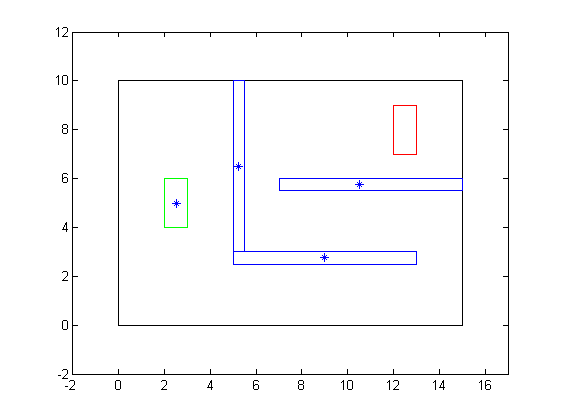
\includegraphics[scale = 0.5]{riddleB}
\caption{Riddle which needs backward step to be solved.}
\end{figure}
\begin{table}[H]
\centering
\begin{tabular}{l||c|c|c}
& \multicolumn{3}{c||}{6 objects} \\\hline\hline
Algorithm& fastest & slowest & medium \\\hline
fList  &  34234 &  35599 & 34917 \\
fList with cells & 24.036 & 27.8225 & 25.001 \\
\end{tabular}
\caption{Time in seconds for counterheuristic riddle.}
\end{table}


%    min 34234
%    max 35599
%    avg 34917
% times for riddleB with function implementation

% min 24.0345
% avg 25.001
% max 27.8225
% time for riddleB with cell function implementation

\section{Interpretation}
As we can see the algorithm working with functions is much faster. But still it scales with an increasing amount of objects to work with.
If we plot these two against each other we see an exponential grow depending on the number of objects involved for the pList algorithm.
The fList algorithms still scale with the number of objects, but are more dependent on the initial positioning of the objects.
\begin{figure}[H]
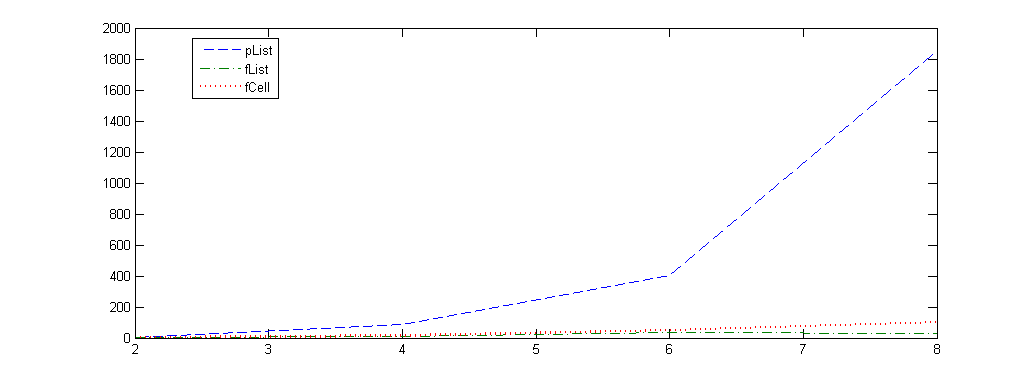
\includegraphics[width=\textwidth]{pointAgainstFuncAgainstCell.png}
\caption{ Plot of the tree algorithms showing the time needed to finish depending on the objects involved.}
\end{figure}
It can easily be seen, that the algorithm pList with point list representation scales extremely bad with an increasing number of objects. This is due to the fact that not only the objects in the direct way beetween target and starting point are considered, but also the extended vectors of objects that are not in the way. This leads to increased number of cells to search through.
\begin{figure}[H]
\centering
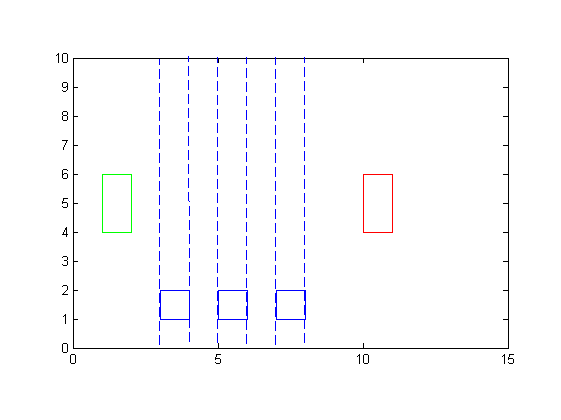
\includegraphics[width=\textwidth, height=250pt]{ghostplanesStep}
\caption{Plot showing the ghostplanes between main object and target.}
\end{figure}
In this plot we can see that there are 6 ghostplanes, extending from the borders of the obstacles in blue, beetween the main object in green and the target in red. Due to this $6\cdot2 = 12$ unnecessary steps need to be calculated before the final step, as per plane we calculate a position in front and behind before evaluating which position is better.\\
If this scenario is given to the algorithm $fList$ ( $fCell$ ) with functions, it would simply check if the obstacles on the bottom are in the way. And as that is not the case, no unecessary steps would arise and the algorithm woud finish in 1 step.\\
\newline
Concerning the counterheuristic riddle the data shows that the algorithm $fCell$ is around $1400$ times faster than the simpler $fList$ algorithm. The algorithm with $pList$ is not listed here, as it takes more than $16h = 57600$ to finish. The calculation was abonded at that time.\\
Comparing the two algorithms $fList$ and $fCel$l, it can be seen that $fList$ is faster for normal calculations with many objects, but fails if the heuristik is bad in the pathplanning. \\
$fCel$l on the other hand reduces the number of cells, thus decreasing the number of steps for the pathplanning. This shortens the path in a way, such that fewer steps in the wrong direction need to be taken to find the target. So for a general purpose algorithm, $fCell$ would be the best choice as it takes only a small penalty for more objects added compared to $fList$, but can deal better with hard riddles.